\documentclass[twocolumn]{article}
\usepackage{graphicx}
\usepackage{amsmath}

\begin{document}
\title{Final Exam: Inverse iteration algorithm for eigenvalues}
\author{Simon Vendelbo Bylling Jensen\thanks{AU E-mail: 201507956@uni.au.dk} \thanks{CERN E-mail: simon.vendelbo.jensen@cern.ch}\\
Stud. Nr. 201507956 \\
Au Id. Au545766}
\date{\today}
\maketitle

\begin{abstract}
The  solution of exercise 10 for the final exam. An implementation f an inverse iteration algorithm for eigenvalues and eigenvectors. Such an implementation has been made, the first relying on a Golub-Kahan-Lanczos bidiagonalization iterating using a calculated inverse of the matrix, as well as a method using QR-decomposition by modified Gram-Schmidt orthogonalization to iterate through the solution of a linear system using backsubstitution. 
\end{abstract}

\section*{Introduction and Problem description}
I have recieved exercise number 10, since my student number 56 by modulus 23 will give 10. The problem is to implement a variant of the inverse iteration method that calculates the eigenvalue closest to a given number $s$ and the corresponding eigenvector. The problem of finding eigenvalues and corresponding eigenvectors are crucial to various fields of physics and engineering. Especially for higly complicated quantum systems, complicated enginerring systems and much more, the task of finding an individual eigenvalue and determine its corresponding eigenvectors is essential. The algorithm, which will be demonstrated is a fast and effective way of doing excactly that. 

At first the implementation and theory of inverse iteration method the will be described in section \ref{sec:0} and afterwards the different related methods will be compared and analysed in section \ref{sec:5}. Implementations and simple calculations using the examined methods will similarly be demonstrated in the main.c file, and which results can be found in the out.txt file, as well as described hereafter. 

\section{\label{sec:0}Implementation and Theory}
The implementation and theory all relies on the lecture notes from ref. \cite[Chapter 12 - Eigenvalues 2: Power methods and Krylov subspace methods]{Dmi}. The refined inverse iteration method relies on a few simple principles. All of these principles will be described by different examples, which are all demonstrated in the main.c file, and which results can be found in the out.txt file. The description of the inverse iteration method will thereby be clear, by going through simpler implementations of the same procedure. This will be the case for sections \ref{sec:1, sec:2}. Hereafter first the implementation using a Golub-Kahan-Lanczos bidiagonalization will be described in section \ref{sec:3} at at last, the refined incerse iteration method will be described in section \ref{sec:4}.  

\subsection{\label{sec:1}The Power Method}
Since the inverse iteration method is a cleverly designed power method, it is essential to introduce the basics of the power methods. The simplest power method is the power iteration which works by multiplying a random vector $\vec{V}$ on a matrix $A$ of similar size, which we want to know the largest eigenvalue and corresponding eigenvector. By continiously multiplying the vector $\vec{V}$ on the matrix $A$, through the iteration
\begin{equation}
\vec{V}_{i+1} = A \vec{V}_i \label{eq:1}
\end{equation}
we are able to aproximate the largest eigenvector and largest eigenvalue very cleverly. The vector will at some point simply converge to the largest eigenvector. This is since by the multiplication, the dimension in which the eigenvector corresponding to the numerically largest eigenvalue will give the largest enhancement of the vector, $\vec{V}$, and for each iteration, this will have positive feedback and will at some point have $\vec{V}$ converge to some vector, which normalized will approximate that eigenvector. If the vector $\vec{V}$ will converge to the eigenvector, then at some point every iteration and thereby multiplicaltion will fullfill the eigenvector identity
\begin{equation}
\vec{V}_\lambda A = \lambda A
\end{equation}
We will thereby be able to approximate the largest eigenvalue continuously by finding the factor, in which V increases for every iteration. This parameter which are contiously detected are called the Rayleigh quotient, and will at one point converge to the largest eigenvalue. This is given as
\begin{equation}
\lambda \left[ \vec{V}_i \right] = \frac{\vec{V}^T_i A \vec{V}}{\vec{V}_i \cdot \vec{V}_i}
\end{equation}
For the implementation in main.c. the satisfaction critera for when an eigenvalue has been found, is when this Rayleigh quotient have converged and do not improve anymore with an iteration. This method is particularly effective in use, since it do not have to do any large matrix decompositions, which the computation of eigenvalues usually requires. 

\section{\label{sec:2}The Inverse Power method}
Intuitively, when one would be able to converge to the numerical largest eigenvalue by continuisly multiplying with the matrix $A$ one would expect, that a similar procedure could be done to find the numerically smallest eigenvalue. This is true, but the cost of this implementation, is the fact that one would in this case have to calculate the inverse of the matrix $A$. By the similar argument as for the power method, by multiplying with the inverse of $A$, the minimum eigenvalue, will now be dominant and the vector $\vec{V}$ will converge to the corresponding eigenvector. The iterations are hereby similar to equation \eqref{eq:1} and given as
\begin{equation}
\vec{V}_{i+1} = A^{-1} \vec{V}_i \label{eq:4}
\end{equation}

The inverse are for this case, for the implementation as found un 





  \begin{figure}[h]
% GNUPLOT: LaTeX picture with Postscript
\begingroup
  \makeatletter
  \providecommand\color[2][]{%
    \GenericError{(gnuplot) \space\space\space\@spaces}{%
      Package color not loaded in conjunction with
      terminal option `colourtext'%
    }{See the gnuplot documentation for explanation.%
    }{Either use 'blacktext' in gnuplot or load the package
      color.sty in LaTeX.}%
    \renewcommand\color[2][]{}%
  }%
  \providecommand\includegraphics[2][]{%
    \GenericError{(gnuplot) \space\space\space\@spaces}{%
      Package graphicx or graphics not loaded%
    }{See the gnuplot documentation for explanation.%
    }{The gnuplot epslatex terminal needs graphicx.sty or graphics.sty.}%
    \renewcommand\includegraphics[2][]{}%
  }%
  \providecommand\rotatebox[2]{#2}%
  \@ifundefined{ifGPcolor}{%
    \newif\ifGPcolor
    \GPcolortrue
  }{}%
  \@ifundefined{ifGPblacktext}{%
    \newif\ifGPblacktext
    \GPblacktexttrue
  }{}%
  % define a \g@addto@macro without @ in the name:
  \let\gplgaddtomacro\g@addto@macro
  % define empty templates for all commands taking text:
  \gdef\gplbacktext{}%
  \gdef\gplfronttext{}%
  \makeatother
  \ifGPblacktext
    % no textcolor at all
    \def\colorrgb#1{}%
    \def\colorgray#1{}%
  \else
    % gray or color?
    \ifGPcolor
      \def\colorrgb#1{\color[rgb]{#1}}%
      \def\colorgray#1{\color[gray]{#1}}%
      \expandafter\def\csname LTw\endcsname{\color{white}}%
      \expandafter\def\csname LTb\endcsname{\color{black}}%
      \expandafter\def\csname LTa\endcsname{\color{black}}%
      \expandafter\def\csname LT0\endcsname{\color[rgb]{1,0,0}}%
      \expandafter\def\csname LT1\endcsname{\color[rgb]{0,1,0}}%
      \expandafter\def\csname LT2\endcsname{\color[rgb]{0,0,1}}%
      \expandafter\def\csname LT3\endcsname{\color[rgb]{1,0,1}}%
      \expandafter\def\csname LT4\endcsname{\color[rgb]{0,1,1}}%
      \expandafter\def\csname LT5\endcsname{\color[rgb]{1,1,0}}%
      \expandafter\def\csname LT6\endcsname{\color[rgb]{0,0,0}}%
      \expandafter\def\csname LT7\endcsname{\color[rgb]{1,0.3,0}}%
      \expandafter\def\csname LT8\endcsname{\color[rgb]{0.5,0.5,0.5}}%
    \else
      % gray
      \def\colorrgb#1{\color{black}}%
      \def\colorgray#1{\color[gray]{#1}}%
      \expandafter\def\csname LTw\endcsname{\color{white}}%
      \expandafter\def\csname LTb\endcsname{\color{black}}%
      \expandafter\def\csname LTa\endcsname{\color{black}}%
      \expandafter\def\csname LT0\endcsname{\color{black}}%
      \expandafter\def\csname LT1\endcsname{\color{black}}%
      \expandafter\def\csname LT2\endcsname{\color{black}}%
      \expandafter\def\csname LT3\endcsname{\color{black}}%
      \expandafter\def\csname LT4\endcsname{\color{black}}%
      \expandafter\def\csname LT5\endcsname{\color{black}}%
      \expandafter\def\csname LT6\endcsname{\color{black}}%
      \expandafter\def\csname LT7\endcsname{\color{black}}%
      \expandafter\def\csname LT8\endcsname{\color{black}}%
    \fi
  \fi
    \setlength{\unitlength}{0.0500bp}%
    \ifx\gptboxheight\undefined%
      \newlength{\gptboxheight}%
      \newlength{\gptboxwidth}%
      \newsavebox{\gptboxtext}%
    \fi%
    \setlength{\fboxrule}{0.5pt}%
    \setlength{\fboxsep}{1pt}%
\begin{picture}(4320.00,3456.00)%
    \gplgaddtomacro\gplbacktext{%
      \csname LTb\endcsname%%
      \put(645,669){\makebox(0,0)[r]{\strut{}$0$}}%
      \csname LTb\endcsname%%
      \put(645,994){\makebox(0,0)[r]{\strut{}$100$}}%
      \csname LTb\endcsname%%
      \put(645,1319){\makebox(0,0)[r]{\strut{}$200$}}%
      \csname LTb\endcsname%%
      \put(645,1644){\makebox(0,0)[r]{\strut{}$300$}}%
      \csname LTb\endcsname%%
      \put(645,1969){\makebox(0,0)[r]{\strut{}$400$}}%
      \csname LTb\endcsname%%
      \put(645,2294){\makebox(0,0)[r]{\strut{}$500$}}%
      \csname LTb\endcsname%%
      \put(645,2619){\makebox(0,0)[r]{\strut{}$600$}}%
      \csname LTb\endcsname%%
      \put(645,2944){\makebox(0,0)[r]{\strut{}$700$}}%
      \csname LTb\endcsname%%
      \put(645,3269){\makebox(0,0)[r]{\strut{}$800$}}%
      \csname LTb\endcsname%%
      \put(821,409){\makebox(0,0){\strut{}$0$}}%
      \csname LTb\endcsname%%
      \put(1341,409){\makebox(0,0){\strut{}$5$}}%
      \csname LTb\endcsname%%
      \put(1860,409){\makebox(0,0){\strut{}$10$}}%
      \csname LTb\endcsname%%
      \put(2380,409){\makebox(0,0){\strut{}$15$}}%
      \csname LTb\endcsname%%
      \put(2900,409){\makebox(0,0){\strut{}$20$}}%
      \csname LTb\endcsname%%
      \put(3419,409){\makebox(0,0){\strut{}$25$}}%
      \csname LTb\endcsname%%
      \put(3939,409){\makebox(0,0){\strut{}$30$}}%
    }%
    \gplgaddtomacro\gplfronttext{%
      \csname LTb\endcsname%%
      \put(153,1969){\rotatebox{-270}{\makebox(0,0){\strut{}Number of Iterations}}}%
      \csname LTb\endcsname%%
      \put(2380,130){\makebox(0,0){\strut{}Matrix Dimension "n"}}%
      \csname LTb\endcsname%%
      \put(3065,3102){\makebox(0,0)[r]{\strut{}Power Iter.}}%
      \csname LTb\endcsname%%
      \put(3065,2916){\makebox(0,0)[r]{\strut{}Inverse Power Iter.}}%
      \csname LTb\endcsname%%
      \put(3065,2730){\makebox(0,0)[r]{\strut{}Shifted Inverse Iter.}}%
      \csname LTb\endcsname%%
      \put(3065,2544){\makebox(0,0)[r]{\strut{}Inverse Iter.}}%
    }%
    \gplbacktext
    \put(0,0){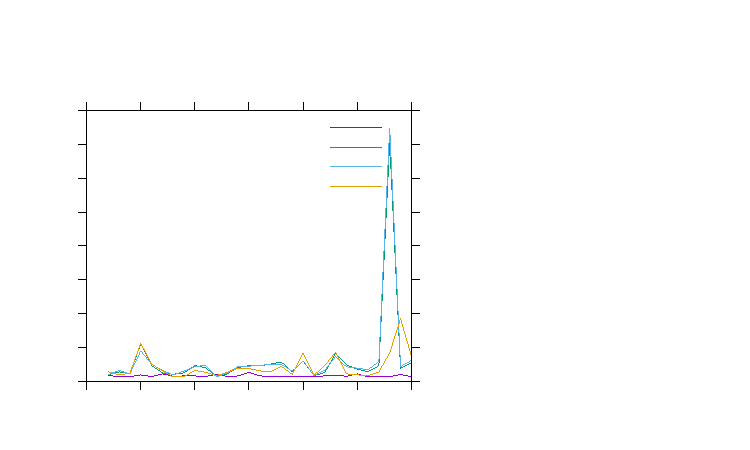
\includegraphics{plot-cairo}}%
    \gplfronttext
  \end{picture}%
\endgroup

\caption{Comparison between the calculated arctangent function using the differential equation found in "myarctan.c" and the arctangent function from the math.h library.}
\label{fig-atan}
\end{figure}

  \begin{figure}[h]
% GNUPLOT: LaTeX picture with Postscript
\begingroup
  \makeatletter
  \providecommand\color[2][]{%
    \GenericError{(gnuplot) \space\space\space\@spaces}{%
      Package color not loaded in conjunction with
      terminal option `colourtext'%
    }{See the gnuplot documentation for explanation.%
    }{Either use 'blacktext' in gnuplot or load the package
      color.sty in LaTeX.}%
    \renewcommand\color[2][]{}%
  }%
  \providecommand\includegraphics[2][]{%
    \GenericError{(gnuplot) \space\space\space\@spaces}{%
      Package graphicx or graphics not loaded%
    }{See the gnuplot documentation for explanation.%
    }{The gnuplot epslatex terminal needs graphicx.sty or graphics.sty.}%
    \renewcommand\includegraphics[2][]{}%
  }%
  \providecommand\rotatebox[2]{#2}%
  \@ifundefined{ifGPcolor}{%
    \newif\ifGPcolor
    \GPcolortrue
  }{}%
  \@ifundefined{ifGPblacktext}{%
    \newif\ifGPblacktext
    \GPblacktexttrue
  }{}%
  % define a \g@addto@macro without @ in the name:
  \let\gplgaddtomacro\g@addto@macro
  % define empty templates for all commands taking text:
  \gdef\gplbacktext{}%
  \gdef\gplfronttext{}%
  \makeatother
  \ifGPblacktext
    % no textcolor at all
    \def\colorrgb#1{}%
    \def\colorgray#1{}%
  \else
    % gray or color?
    \ifGPcolor
      \def\colorrgb#1{\color[rgb]{#1}}%
      \def\colorgray#1{\color[gray]{#1}}%
      \expandafter\def\csname LTw\endcsname{\color{white}}%
      \expandafter\def\csname LTb\endcsname{\color{black}}%
      \expandafter\def\csname LTa\endcsname{\color{black}}%
      \expandafter\def\csname LT0\endcsname{\color[rgb]{1,0,0}}%
      \expandafter\def\csname LT1\endcsname{\color[rgb]{0,1,0}}%
      \expandafter\def\csname LT2\endcsname{\color[rgb]{0,0,1}}%
      \expandafter\def\csname LT3\endcsname{\color[rgb]{1,0,1}}%
      \expandafter\def\csname LT4\endcsname{\color[rgb]{0,1,1}}%
      \expandafter\def\csname LT5\endcsname{\color[rgb]{1,1,0}}%
      \expandafter\def\csname LT6\endcsname{\color[rgb]{0,0,0}}%
      \expandafter\def\csname LT7\endcsname{\color[rgb]{1,0.3,0}}%
      \expandafter\def\csname LT8\endcsname{\color[rgb]{0.5,0.5,0.5}}%
    \else
      % gray
      \def\colorrgb#1{\color{black}}%
      \def\colorgray#1{\color[gray]{#1}}%
      \expandafter\def\csname LTw\endcsname{\color{white}}%
      \expandafter\def\csname LTb\endcsname{\color{black}}%
      \expandafter\def\csname LTa\endcsname{\color{black}}%
      \expandafter\def\csname LT0\endcsname{\color{black}}%
      \expandafter\def\csname LT1\endcsname{\color{black}}%
      \expandafter\def\csname LT2\endcsname{\color{black}}%
      \expandafter\def\csname LT3\endcsname{\color{black}}%
      \expandafter\def\csname LT4\endcsname{\color{black}}%
      \expandafter\def\csname LT5\endcsname{\color{black}}%
      \expandafter\def\csname LT6\endcsname{\color{black}}%
      \expandafter\def\csname LT7\endcsname{\color{black}}%
      \expandafter\def\csname LT8\endcsname{\color{black}}%
    \fi
  \fi
    \setlength{\unitlength}{0.0500bp}%
    \ifx\gptboxheight\undefined%
      \newlength{\gptboxheight}%
      \newlength{\gptboxwidth}%
      \newsavebox{\gptboxtext}%
    \fi%
    \setlength{\fboxrule}{0.5pt}%
    \setlength{\fboxsep}{1pt}%
\begin{picture}(4320.00,3456.00)%
    \gplgaddtomacro\gplbacktext{%
      \csname LTb\endcsname%%
      \put(543,669){\makebox(0,0)[r]{\strut{}$10$}}%
      \csname LTb\endcsname%%
      \put(543,975){\makebox(0,0)[r]{\strut{}$20$}}%
      \csname LTb\endcsname%%
      \put(543,1281){\makebox(0,0)[r]{\strut{}$30$}}%
      \csname LTb\endcsname%%
      \put(543,1587){\makebox(0,0)[r]{\strut{}$40$}}%
      \csname LTb\endcsname%%
      \put(543,1893){\makebox(0,0)[r]{\strut{}$50$}}%
      \csname LTb\endcsname%%
      \put(543,2198){\makebox(0,0)[r]{\strut{}$60$}}%
      \csname LTb\endcsname%%
      \put(543,2504){\makebox(0,0)[r]{\strut{}$70$}}%
      \csname LTb\endcsname%%
      \put(543,2810){\makebox(0,0)[r]{\strut{}$80$}}%
      \csname LTb\endcsname%%
      \put(543,3116){\makebox(0,0)[r]{\strut{}$90$}}%
      \csname LTb\endcsname%%
      \put(719,409){\makebox(0,0){\strut{}$2$}}%
      \csname LTb\endcsname%%
      \put(1179,409){\makebox(0,0){\strut{}$3$}}%
      \csname LTb\endcsname%%
      \put(1639,409){\makebox(0,0){\strut{}$4$}}%
      \csname LTb\endcsname%%
      \put(2099,409){\makebox(0,0){\strut{}$5$}}%
      \csname LTb\endcsname%%
      \put(2559,409){\makebox(0,0){\strut{}$6$}}%
      \csname LTb\endcsname%%
      \put(3019,409){\makebox(0,0){\strut{}$7$}}%
      \csname LTb\endcsname%%
      \put(3479,409){\makebox(0,0){\strut{}$8$}}%
      \csname LTb\endcsname%%
      \put(3939,409){\makebox(0,0){\strut{}$9$}}%
    }%
    \gplgaddtomacro\gplfronttext{%
      \csname LTb\endcsname%%
      \put(153,1969){\rotatebox{-270}{\makebox(0,0){\strut{}Number of iterations}}}%
      \csname LTb\endcsname%%
      \put(2329,130){\makebox(0,0){\strut{}Matrix Dimension "n"}}%
      \csname LTb\endcsname%%
      \put(2657,3102){\makebox(0,0)[r]{\strut{}20 Iter. per. Upd.}}%
      \csname LTb\endcsname%%
      \put(2657,2916){\makebox(0,0)[r]{\strut{}40 Iter. per. Upd.}}%
      \csname LTb\endcsname%%
      \put(2657,2730){\makebox(0,0)[r]{\strut{}60 Iter. per. Upd.}}%
      \csname LTb\endcsname%%
      \put(2657,2544){\makebox(0,0)[r]{\strut{}80 Iter. per. Upd.}}%
    }%
    \gplbacktext
    \put(0,0){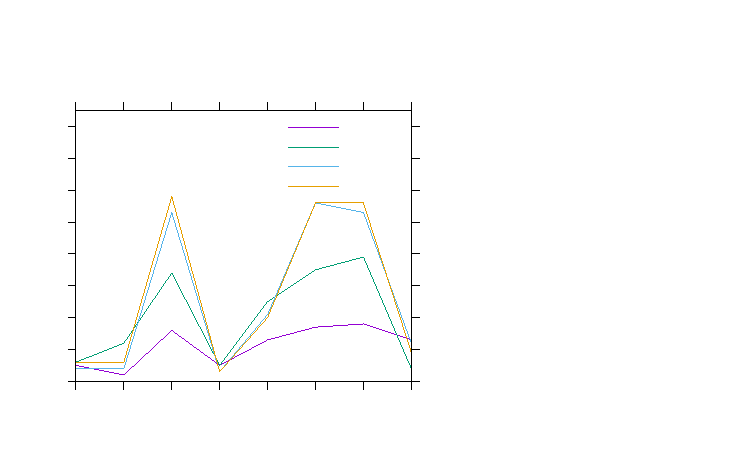
\includegraphics{plot-cairo-2}}%
    \gplfronttext
  \end{picture}%
\endgroup

\caption{Comparison between the calculated arctangent function using the differential equation found in "myarctan.c" and the arctangent function from the math.h library.}
\label{fig-atan}
\end{figure}


\begin{figure}[h]
% GNUPLOT: LaTeX picture with Postscript
\begingroup
  \makeatletter
  \providecommand\color[2][]{%
    \GenericError{(gnuplot) \space\space\space\@spaces}{%
      Package color not loaded in conjunction with
      terminal option `colourtext'%
    }{See the gnuplot documentation for explanation.%
    }{Either use 'blacktext' in gnuplot or load the package
      color.sty in LaTeX.}%
    \renewcommand\color[2][]{}%
  }%
  \providecommand\includegraphics[2][]{%
    \GenericError{(gnuplot) \space\space\space\@spaces}{%
      Package graphicx or graphics not loaded%
    }{See the gnuplot documentation for explanation.%
    }{The gnuplot epslatex terminal needs graphicx.sty or graphics.sty.}%
    \renewcommand\includegraphics[2][]{}%
  }%
  \providecommand\rotatebox[2]{#2}%
  \@ifundefined{ifGPcolor}{%
    \newif\ifGPcolor
    \GPcolortrue
  }{}%
  \@ifundefined{ifGPblacktext}{%
    \newif\ifGPblacktext
    \GPblacktexttrue
  }{}%
  % define a \g@addto@macro without @ in the name:
  \let\gplgaddtomacro\g@addto@macro
  % define empty templates for all commands taking text:
  \gdef\gplbacktext{}%
  \gdef\gplfronttext{}%
  \makeatother
  \ifGPblacktext
    % no textcolor at all
    \def\colorrgb#1{}%
    \def\colorgray#1{}%
  \else
    % gray or color?
    \ifGPcolor
      \def\colorrgb#1{\color[rgb]{#1}}%
      \def\colorgray#1{\color[gray]{#1}}%
      \expandafter\def\csname LTw\endcsname{\color{white}}%
      \expandafter\def\csname LTb\endcsname{\color{black}}%
      \expandafter\def\csname LTa\endcsname{\color{black}}%
      \expandafter\def\csname LT0\endcsname{\color[rgb]{1,0,0}}%
      \expandafter\def\csname LT1\endcsname{\color[rgb]{0,1,0}}%
      \expandafter\def\csname LT2\endcsname{\color[rgb]{0,0,1}}%
      \expandafter\def\csname LT3\endcsname{\color[rgb]{1,0,1}}%
      \expandafter\def\csname LT4\endcsname{\color[rgb]{0,1,1}}%
      \expandafter\def\csname LT5\endcsname{\color[rgb]{1,1,0}}%
      \expandafter\def\csname LT6\endcsname{\color[rgb]{0,0,0}}%
      \expandafter\def\csname LT7\endcsname{\color[rgb]{1,0.3,0}}%
      \expandafter\def\csname LT8\endcsname{\color[rgb]{0.5,0.5,0.5}}%
    \else
      % gray
      \def\colorrgb#1{\color{black}}%
      \def\colorgray#1{\color[gray]{#1}}%
      \expandafter\def\csname LTw\endcsname{\color{white}}%
      \expandafter\def\csname LTb\endcsname{\color{black}}%
      \expandafter\def\csname LTa\endcsname{\color{black}}%
      \expandafter\def\csname LT0\endcsname{\color{black}}%
      \expandafter\def\csname LT1\endcsname{\color{black}}%
      \expandafter\def\csname LT2\endcsname{\color{black}}%
      \expandafter\def\csname LT3\endcsname{\color{black}}%
      \expandafter\def\csname LT4\endcsname{\color{black}}%
      \expandafter\def\csname LT5\endcsname{\color{black}}%
      \expandafter\def\csname LT6\endcsname{\color{black}}%
      \expandafter\def\csname LT7\endcsname{\color{black}}%
      \expandafter\def\csname LT8\endcsname{\color{black}}%
    \fi
  \fi
    \setlength{\unitlength}{0.0500bp}%
    \ifx\gptboxheight\undefined%
      \newlength{\gptboxheight}%
      \newlength{\gptboxwidth}%
      \newsavebox{\gptboxtext}%
    \fi%
    \setlength{\fboxrule}{0.5pt}%
    \setlength{\fboxsep}{1pt}%
\begin{picture}(4320.00,2592.00)%
    \gplgaddtomacro\gplbacktext{%
      \csname LTb\endcsname%%
      \put(645,669){\makebox(0,0)[r]{\strut{}$0$}}%
      \csname LTb\endcsname%%
      \put(645,862){\makebox(0,0)[r]{\strut{}$0.5$}}%
      \csname LTb\endcsname%%
      \put(645,1055){\makebox(0,0)[r]{\strut{}$1$}}%
      \csname LTb\endcsname%%
      \put(645,1248){\makebox(0,0)[r]{\strut{}$1.5$}}%
      \csname LTb\endcsname%%
      \put(645,1441){\makebox(0,0)[r]{\strut{}$2$}}%
      \csname LTb\endcsname%%
      \put(645,1633){\makebox(0,0)[r]{\strut{}$2.5$}}%
      \csname LTb\endcsname%%
      \put(645,1826){\makebox(0,0)[r]{\strut{}$3$}}%
      \csname LTb\endcsname%%
      \put(645,2019){\makebox(0,0)[r]{\strut{}$3.5$}}%
      \csname LTb\endcsname%%
      \put(645,2212){\makebox(0,0)[r]{\strut{}$4$}}%
      \csname LTb\endcsname%%
      \put(645,2405){\makebox(0,0)[r]{\strut{}$4.5$}}%
      \csname LTb\endcsname%%
      \put(821,409){\makebox(0,0){\strut{}$100$}}%
      \csname LTb\endcsname%%
      \put(1266,409){\makebox(0,0){\strut{}$200$}}%
      \csname LTb\endcsname%%
      \put(1712,409){\makebox(0,0){\strut{}$300$}}%
      \csname LTb\endcsname%%
      \put(2157,409){\makebox(0,0){\strut{}$400$}}%
      \csname LTb\endcsname%%
      \put(2603,409){\makebox(0,0){\strut{}$500$}}%
      \csname LTb\endcsname%%
      \put(3048,409){\makebox(0,0){\strut{}$600$}}%
      \csname LTb\endcsname%%
      \put(3494,409){\makebox(0,0){\strut{}$700$}}%
      \csname LTb\endcsname%%
      \put(3939,409){\makebox(0,0){\strut{}$800$}}%
    }%
    \gplgaddtomacro\gplfronttext{%
      \csname LTb\endcsname%%
      \put(153,1537){\rotatebox{-270}{\makebox(0,0){\strut{}y}}}%
      \csname LTb\endcsname%%
      \put(2380,130){\makebox(0,0){\strut{}x}}%
      \csname LTb\endcsname%%
      \put(2657,2238){\makebox(0,0)[r]{\strut{}Inverse Iteration}}%
      \csname LTb\endcsname%%
      \put(2657,2052){\makebox(0,0)[r]{\strut{}Jacobi Diag.}}%
    }%
    \gplbacktext
    \put(0,0){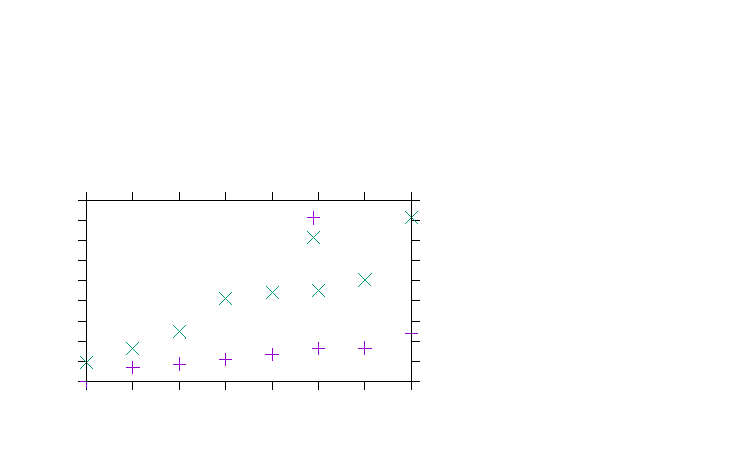
\includegraphics{plot-cairo_time}}%
    \gplfronttext
  \end{picture}%
\endgroup

\caption{Examination of the computing time as a function of....}
\label{fig-atan}
\end{figure}

\begin{thebibliography}{9}

\bibitem{Dmi}
  Fedorov, D.V.
  \textit{Introduction to Numercal Methods},
  Lecture Notes, Aarhus University,
  2019.

\end{thebibliography}

\end{document}
